\documentclass[tikz]{standalone}

\usetikzlibrary{arrows}
\usetikzlibrary{arrows.meta}

\begin{document}

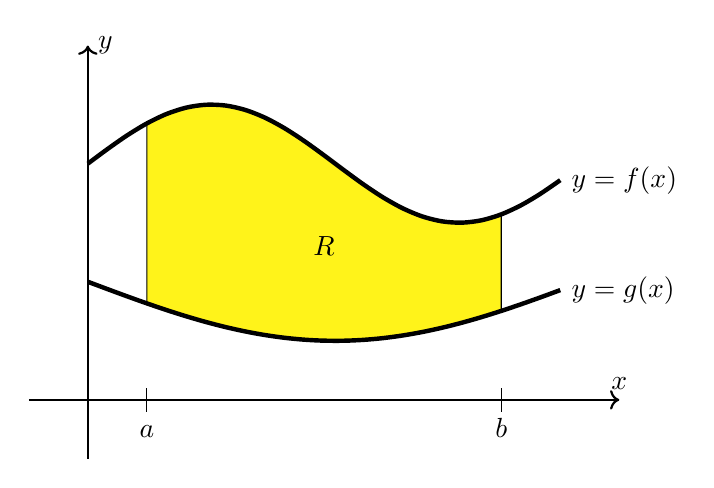
\begin{tikzpicture}[scale=1.5]
      
    % shade region
    \draw[smooth,fill=yellow!90] plot[domain=0.5:3.5] ({\x},{2 + 0.5*sin(1.5*\x r)}) --
    plot[domain=3.5:0.5] ({\x},{1 - 0.5*sin(0.75*\x r)}) -- cycle;
  
    % draw axes
    \draw[thick,->] (-0.5,0) -- (4.5,0) node[above] {$x$};
    \draw[thick,->] (0,-0.5) -- (0,3) node[right] {$y$};
  
    % draw curve
    \draw[ultra thick,domain=0:4,smooth] plot ({\x},{2 + 0.5*sin(1.5*\x r)}) node[right] {$y=f(x)$};
    \draw[ultra thick,domain=0:4,smooth] plot ({\x},{1 - 0.5*sin(0.75*\x r)}) node[right] {$y=g(x)$};
  
    \draw (0.5,0.1) -- (0.5,-0.1);
    \draw (0.5,-0.4) node[above] {$a$};
    \draw (3.5,0.1) -- (3.5,-0.1);
    \draw (3.5,-0.4) node[above] {$b$};
  
    \node at (2,1.3) {$R$};
      
\end{tikzpicture}


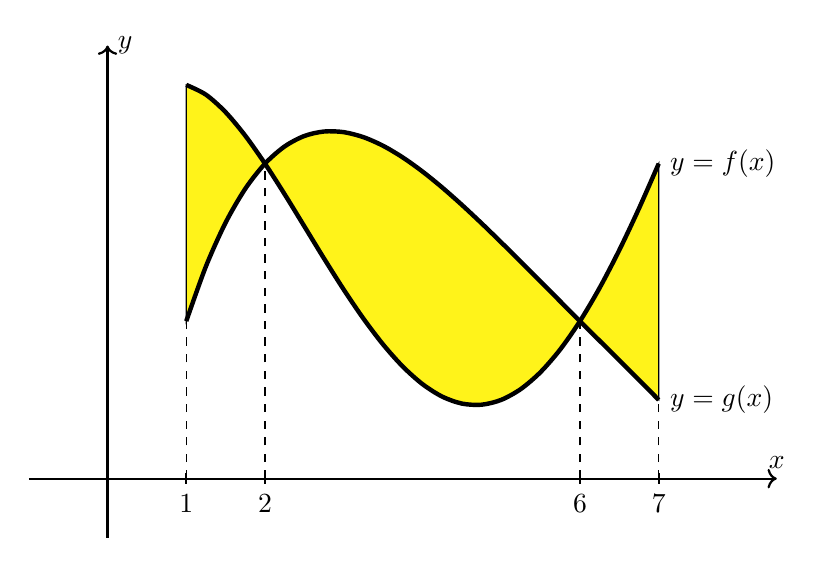
\begin{tikzpicture}

    % shade region
    \draw[smooth,fill=yellow!90] 
    plot[domain=1:7] ({\x},{-5/2 + (61*\x)/10 - (43*\x^2)/24 + \x^3/5 - \x^4/120}) --
    plot[domain=7:1] ({\x},{4 + (77*\x)/30 - (113*\x^2)/60 + \x^3/3 - \x^4/60}) -- cycle;
  
    % draw axes
    \draw[thick,->] (-1,0) -- (8.5,0) node[above] {$x$};
    \draw[thick,->] (0,-0.75) -- (0,5.5) node[right] {$y$};
  
    % draw curves
    \draw[ultra thick,domain=1:7,smooth,variable=\x,black] 
    plot ({\x},{-5/2 + (61*\x)/10 - (43*\x^2)/24 + \x^3/5 - \x^4/120}) node[right] {$y=g(x)$};
    \draw[ultra thick,domain=1:7,smooth,variable=\x,black] 
    plot ({\x},{4 + (77*\x)/30 - (113*\x^2)/60 + \x^3/3 - \x^4/60}) node[right] {$y=f(x)$};
  
    % tick marks
    \foreach \x in {1,2,6,7} 
      \draw [thick] (\x cm,2pt) -- (\x cm,-2pt) node[below] {$\x$};
      
    \draw[dashed] (1,0) -- (1,2);
    \draw[dashed] (2,0) -- (2,4);
    \draw[dashed] (6,0) -- (6,2.1);
    \draw[dashed] (7,0) -- (7,1);
  
\end{tikzpicture}


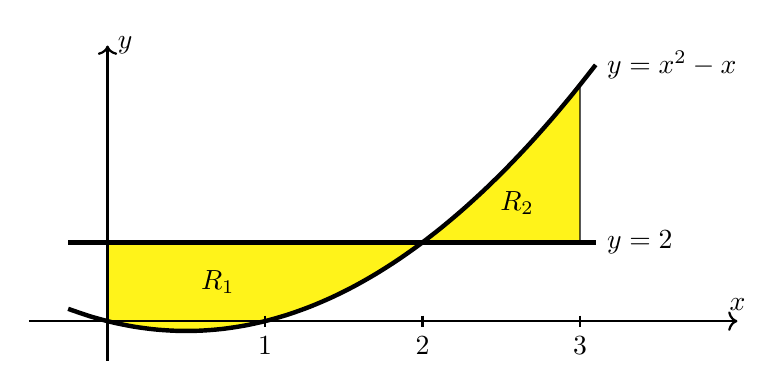
\begin{tikzpicture}[xscale=2.0,yscale=0.5]

    % \draw[fill=white] (-0.75,-1.5) rectangle ++(5,9);
  
    % shade region
    \draw[fill=yellow!90] (0,2) -- plot[domain=0:3,smooth,variable=\x,black] ({\x},{\x* (\x -1)}) |- (0,2);
  
    % draw axes
    \draw[thick,->] (-0.5,0) -- (4,0) node[above] {$x$};
    \draw[thick,->] (0,-1) -- (0,7) node[right] {$y$};
  
    % draw curves
    \draw[ultra thick,domain=-0.25:3.1,smooth,variable=\x,black] plot ({\x},{\x* (\x -1)}) node[right] {$y=x^2-x$};
    \draw[ultra thick,domain=-0.25:3.1,smooth,variable=\x,black] plot ({\x},{2}) node[right] {$y=2$};
    %\draw[ultra thick,domain=-2.3:2.3,smooth,variable=\x,black] plot (\x,\x*\x*\x) node[right] {$y=x^3$};
  
  
    \draw (0.7, 1) node {$R_1$};
    \draw (2.6, 3.0) node {$R_2$};
          
    % tick marks
    \foreach \x in {1,2,3} 
      \draw [thick] (\x cm,4pt) -- (\x cm,-4pt) node[below] {$\x$};
  
\end{tikzpicture}

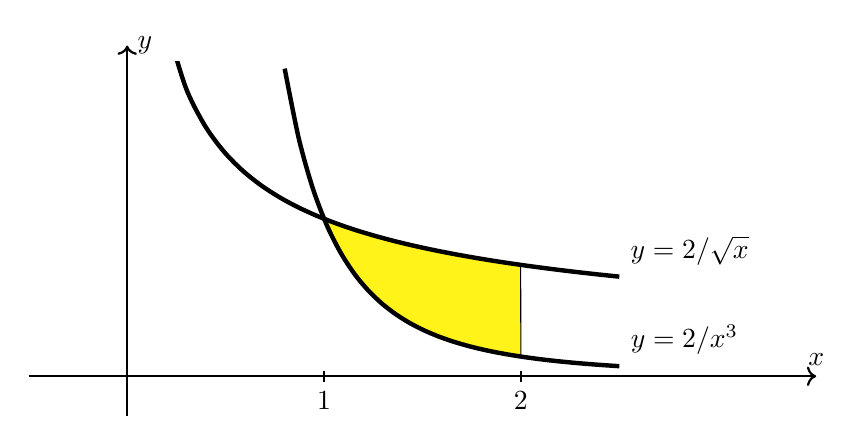
\begin{tikzpicture}[xscale=2.5]

    % \draw[fill=white] (-0.75,-1) rectangle ++(4.5,6);
  
    % shade region
    \draw[fill=yellow!90] plot[smooth, samples=100, domain=1:2] ({\x},{2 / \x^0.5}) -- plot[smooth, samples=100, domain=2:1] ({\x},{2 / \x^3});
  
    %draw axes
    \draw[thick,->] (-0.5,0) -- (3.5,0) node[above] {$x$};
    \draw[thick,->] (0,-0.5) -- (0,4.2) node[right] {$y$};
  
    % draw curves
    \clip (0,-0.5) rectangle ++(3.4,4.5);
    \draw[ultra thick,domain=0.2:2.5,smooth,variable=\x,black] plot ({\x},{2 / \x^0.5}) node[above right] {$y=2/\sqrt{x}$};
    \draw[ultra thick,domain=0.8:2.5,smooth,variable=\x,black] plot ({\x},{2 / \x^3}) node[above right] {$y=2/x^3$};
  
    % tick marks
    \foreach \x in {1,2} 
      \draw [thick] (\x cm,2pt) -- (\x cm,-2pt) node[below] {$\x$};
  
\end{tikzpicture}

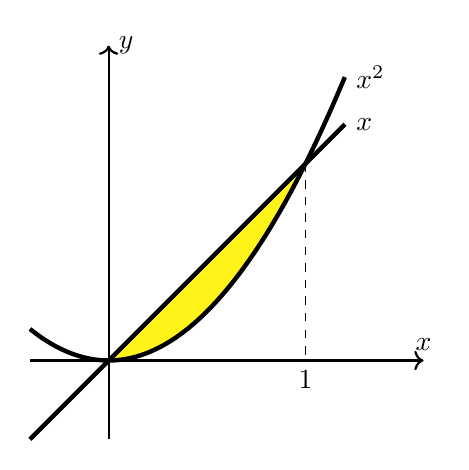
\begin{tikzpicture}
    % \draw[fill=white] (-1.5,-1.5) rectangle ++(6,6);
  
    % shade region
    \draw[fill=yellow!90] plot[smooth, samples=100, domain=0:2.5 ] (\x,0.4*\x*\x) -- (0,0) -- cycle;
  
    % draw axes
    \draw[thick,->] (-1,0) -- (4,0) node[above] {$x$};
    \draw[thick,->] (0,-1) -- (0,4) node[right] {$y$};
  
    % draw curves
    \draw[ultra thick,domain=-1:3,smooth,variable=\x,black] plot ({\x},{0.4*\x*\x}) node[right] {$x^2$};
    \draw[ultra thick, domain=-1:3,smooth,variable=\x,black] plot ({\x},{\x}) node[right] {$x$};
          
    \draw[dashed] (2.5,2.5) -- (2.5,0) node[below] {1};
\end{tikzpicture}

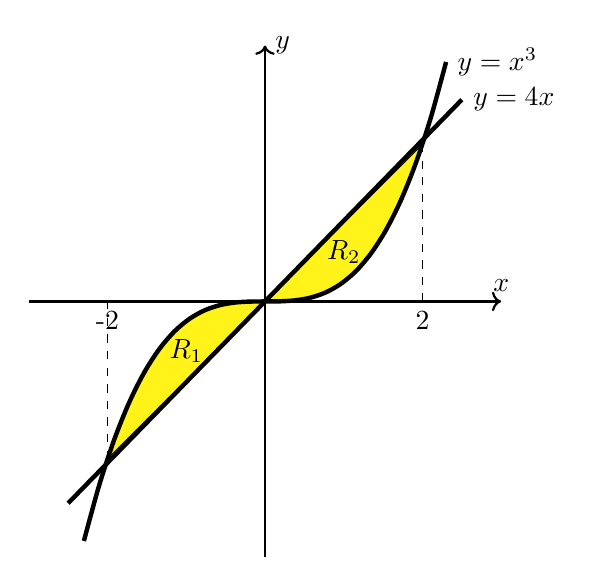
\begin{tikzpicture}[yscale=0.25]
    % \draw[fill=white] (-4,-15) rectangle ++(8,30);
  
    % draw axes
    \draw[thick,->] (-3,0) -- (3,0) node[above] {$x$};
    \draw[thick,->] (0,-13) -- (0,13) node[right] {$y$};
  
    % shade region
    \draw[fill=yellow!90] plot[smooth, samples=100, domain=-2:2] (\x,\x*\x*\x) -- cycle;
  
    % draw curves
    \draw[ultra thick,domain=-2.3:2.3,smooth,variable=\x,black] plot (\x,\x*\x*\x) node[right] {$y=x^3$};
    \draw[ultra thick,domain=-2.5:2.5,smooth,variable=\x,black] plot (\x,4.1*\x) node[right] {$y=4x$};
        
    \draw[dashed] (2,8) -- (2,0) node[below] {2};
    \draw[dashed] (-2,-8) -- (-2,0) node[below] {-2};
  
    \draw (-1, -2.5) node {$R_1$};
    \draw (1, 2.5) node {$R_2$};
\end{tikzpicture}
  



\end{document} 